% OneRec-V2 paper review summary (auto-generated)
\documentclass{article}
\usepackage[margin=1in]{geometry}
\usepackage{graphicx}
\usepackage{hyperref}
\begin{document}

\section*{OneRec-V2 Technical Report (2025)}

\begin{figure}[h]
\centering
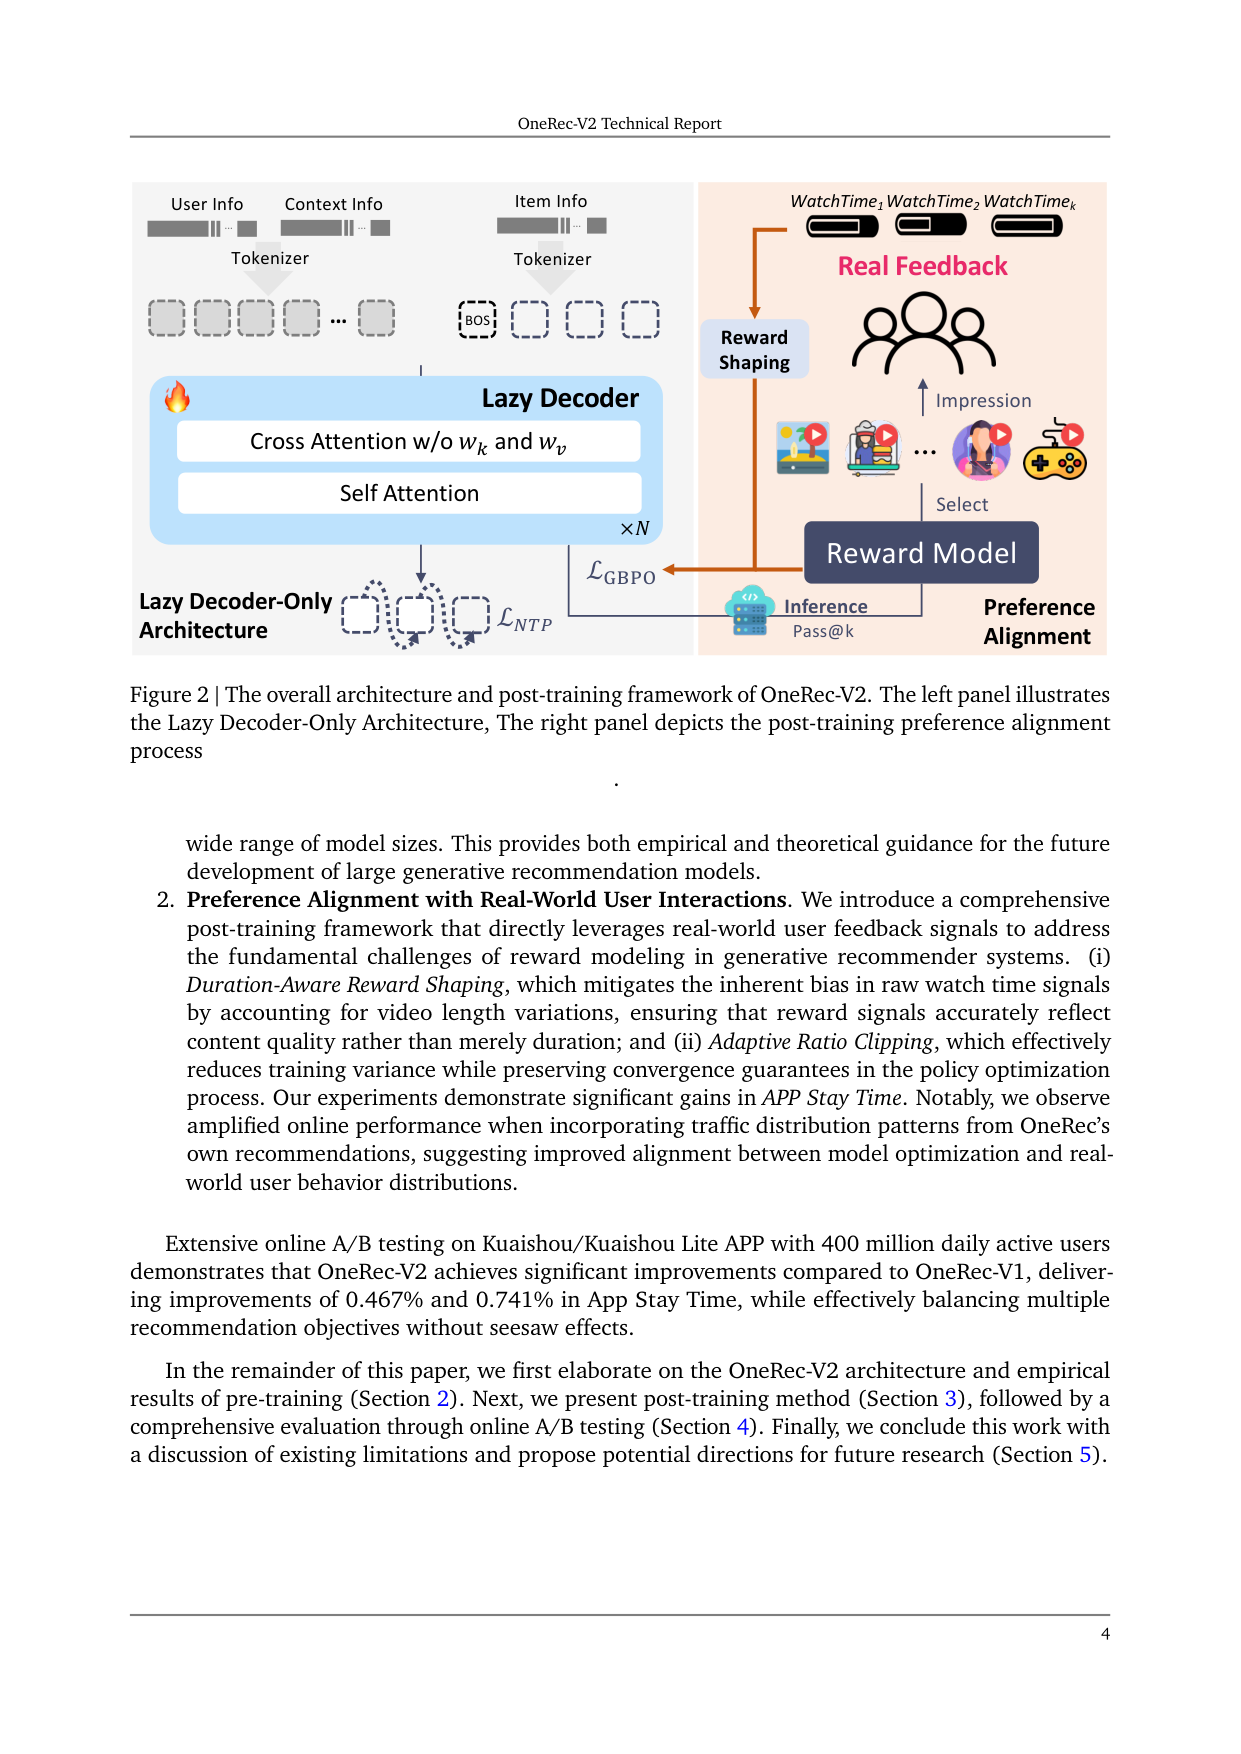
\includegraphics[width=0.95\linewidth]{fig2_overall_architecture.png}
\caption{Overall architecture and post-training framework of OneRec-V2 (paper Figure 2).}
\end{figure}

\subsection*{Challenges}
\begin{itemize}
  \item \textbf{Compute is spent on context encoding, not the loss-relevant generation.} In OneRec-V1's encoder--decoder setup, long user context dominates FLOPs; the paper highlights that with context length 512, \emph{``the context encoding consumes 97.66\% of total FLOPs''} while decoding is only 2.34\%.
  \item \textbf{Scaling bottleneck from architecture imbalance.} Under fixed compute, the encoder-heavy workload limits scaling the generative component where recommendation decisions are made.
  \item \textbf{Reward-model-only RL issues.} Reward-model RL can be sample-inefficient (extra rollout+scoring cost) and vulnerable to reward hacking due to proxy rewards.
  \item \textbf{Using real user feedback is non-trivial.} Raw watch time is biased by video duration; multiple objectives and sparse positives complicate RL from feedback.
\end{itemize}

\subsection*{Key Initiatives}
\begin{itemize}
  \item \textbf{Lazy Decoder-Only Architecture.} Remove the encoder and treat user context as static conditioning accessed via cross-attention, eliminating redundant context computation.
  \item \textbf{Lazy cross-attention without K/V projections + GQA.} Context processor outputs (layer-shared) key/value tensors; decoder blocks apply cross-attention without key/value projection layers and use Grouped Query Attention to reduce memory/IO.
  \item \textbf{Scaling to large models under the same compute.} Reported \emph{``94\% reduction in computational requirements''} and \emph{``90\% reduction in actual training resources''}, enabling scaling up to 8B parameters and observing smooth scaling behavior.
  \item \textbf{Preference alignment from real-world user interactions.} (i) Duration-Aware Reward Shaping to debias watch-time signals; (ii) Gradient-Bounded Policy Optimization (GBPO) with adaptive ratio bounding to stabilize RL.
\end{itemize}

\subsection*{Methodology}
\begin{itemize}
  \item \textbf{Input/target tokenization.} Each item is mapped by a semantic tokenizer to 3 semantic IDs; training uses input \texttt{[BOS, s\_1, s\_2]} and predicts \texttt{[s\_1, s\_2, s\_3]} via autoregressive generation.
  \item \textbf{Context Processor.} Heterogeneous user features (profile + behaviors across pathways) are concatenated into a context sequence and transformed into normalized per-layer key/value pairs \(\{(k_0,v_0),\dots\}\), with configurable key/value sharing across decoder blocks (parameters \(L_{kv}, S_{kv}\)).
  \item \textbf{Lazy Decoder Blocks.} Stack of transformer blocks with: (1) lazy cross-attention to context K/V (often shared across blocks); (2) causal self-attention over the short semantic-token sequence; (3) FFN (with optional MoE in deeper layers).
  \item \textbf{Compute allocation insight.} For lazy decoder-only, target decoding becomes \(\approx 100\%\) of compute regardless of context length (Table 1), versus \(<3\%\) for classic enc--dec/naive dec-only at context length 512.
  \item \textbf{Duration-Aware Reward Shaping.} Bucket each user's historical videos by log-duration \(F(d)=\lfloor \log_{\beta}(d+\epsilon) \rfloor\). For target video \(i\), compute percentile \(q_i\) of its playtime within the corresponding duration bucket, then select positives as top-quartile (and explicit ``dislike'' as negatives).
  \item \textbf{GBPO.} A policy-optimization objective designed to (a) keep gradients from all samples (no ratio clipping drop) while (b) bounding gradients for negative samples with a dynamic bound related to token probability, empirically stabilizing gradient norms versus ECPO/GRPO.
\end{itemize}

\subsection*{Experiments}
\begin{itemize}
  \item \textbf{Architecture efficiency vs loss.} Across 0.1B/0.5B/1B scales, lazy decoder-only matches convergence loss of enc--dec while using far fewer FLOPs and activations (e.g., at 1B: 18.89 GFLOPs and 1.24B activations vs 296.36 GFLOPs and 17.63B activations for enc:dec=1:1; Table 2).
  \item \textbf{Scaling law behavior.} Dense lazy-decoder models from 0.1B\(\to\)8B show decreasing convergence loss 3.57\(\to\)3.19; fitted scaling law \(\hat L(N)=E + A/N^{\alpha}\) with \(E=3.13, A=3660, \alpha=0.489\) (Figure 6).
  \item \textbf{Sparse MoE variant.} 4B total (0.5B active) MoE reaches convergence loss 3.22, outperforming 2B dense while keeping compute similar to 0.5B dense (Table 5 discussion).
  \item \textbf{User-feedback RL (online).} Duration-aware feedback RL improves App Stay Time; adding OneRec-generated samples (on-policy) improves most interaction metrics too (Table 6; e.g., Kuaishou App Stay Time +0.227\%, Video View +0.716\%).
  \item \textbf{Reward model vs user feedback vs hybrid.} Reward model tends to boost interaction metrics more; user feedback tends to boost App Stay Time more; hybrid improves balance (Table 7).
  \item \textbf{Full online A/B test.} 5\% traffic, 1 week; 1B params, context length 3000, beam size 512; L20 GPUs with 36ms latency and MFU 62\%. Reported overall improvements vs OneRec-V1: App Stay Time \emph{``+0.467\%''} (Kuaishou) and \emph{``+0.741\%''} (Kuaishou Lite), with broad gains in interaction metrics (Table 8).
\end{itemize}

\subsection*{References (selected)}
\begin{itemize}
  \item Zhou et al., \emph{OneRec Technical Report}, 2025 (OneRec-V1 baseline).
  \item Hoffmann et al., \emph{Training Compute-Optimal Large Language Models}, 2022 (scaling law).
  \item Ainslie et al., \emph{GQA: Training Generalized Multi-Query Transformer Models}, 2023 (Grouped Query Attention).
  \item Schulman et al., \emph{Proximal Policy Optimization Algorithms}, 2017 (PPO background).
  \item Shao et al., \emph{DeepSeek-Math}, 2024 (GRPO reference in paper).
  \item Liu et al., \emph{DeepSeek-V3 Technical Report}, 2024 (aux-loss-free MoE load balancing reference).
\end{itemize}

\end{document}
